\documentclass[11pt]{book}

\usepackage[authoryear]{natbib}
\usepackage{xcolor}
\usepackage[T1]{fontenc}
\usepackage{fourier}
\usepackage[utf8]{inputenc}
\usepackage[hidelinks]{hyperref}
\usepackage{slashbox}
\usepackage{graphicx}
\usepackage{url}
\usepackage{enumitem}


\newcommand{\todo}[1]{\textcolor{red}{[TODO: #1]}\PackageWarning{TODO:}{#1!}}
\newcommand{\note}[1]{\textcolor{red}{[NOTE: #1]}\PackageWarning{NOTE:}{#1!}}
\newcommand*{\np}{\par\noindent\newline}

\title{Agent Based Modelling of the Formation of Social Preferences}
\author{S Pardy}
\begin{document}
\begin{titlepage}
	\newcommand{\HRule}{\rule{\linewidth}{0.5mm}} % Defines a new command for horizontal lines, change thickness here
	
	\center % Centre everything on the page
	
	%------------------------------------------------
	%	Headings
	%------------------------------------------------
	
	\textsc{\LARGE Monash University}\\[1.5cm]	
	\textsc{\Large Bachelor of Science (Honours)}\\[0.5cm] % Major heading such as course name
	
	\textsc{\large Computational Science}\\[0.5cm] % Minor heading such as course title
	
	%------------------------------------------------
	%	Title
	%------------------------------------------------
	
	\HRule\\[0.4cm]
	
	{\huge\bfseries Agent Based Modelling of the Formation of Social Preferences}\\[0.4cm]
	
	\HRule\\[1.5cm]
	
	%------------------------------------------------
	%	Author(s)
	%------------------------------------------------
	
	\begin{minipage}{0.4\textwidth}
		\begin{flushleft}
			\large
			\textit{Author}\\
			Sam \textsc{Pardy}
		\end{flushleft}
	\end{minipage}
	~
	\begin{minipage}{0.4\textwidth}
		\begin{flushright}
			\large 
			\textit{Student ID}\\
		25940783   
		\end{flushright}
	\end{minipage}
	\vfill
	\vfill
	{\large
	\textit{Supervisor}\\
	Dr. Julian \textsc{Garcia}}
	
	%------------------------------------------------
	%	Date
	%------------------------------------------------
	
	\vfill\vfill\vfill % Position the date 3/4 down the remaining page
	
	{\large\today} % Date

	\vfill % Push the date up 1/4 of the remaining page
	
\end{titlepage}
% \hypersetup{colorlinks, citecolor=black, filecolor=black, linkcolor=black urlcolor=black}

\newpage
\chapter*{Declaration}
\chapter*{Abstract}
\chapter*{Acknowledgment}

\tableofcontents
\newpage
\chapter{Introduction}
\section{Preamble}
\section{Motivation \& Objectives}

\chapter{Literature Review}

\chapter{Limitations of Theory \& The Experimental Framework}

The research discussed in the previous chapters suffers from several limitations that affect the usefulness of the conclusions drawn. 
Chiefly, it is static; the conclusions drawn from the work focus on evolutionarily stable strategies as a solution concept.
These conclusions may be meaningful however do not tell us anything about how likely these strategies are to evolve or what circumstances may lead to them evolving.
Further, the work is slightly abstract in that in places it does not detail specific attributes of the model it is working with in favour of broader `catch-all' definitions,
this has made the process of creating a software-based replicas of the models difficult at times.

The experimental framework that we have created as part of `this' research seeks to recreate these models as dynamically-evolving in attempt to recover the static results of existing work.




\chapter{The Model}
\section{To Be Young and Fit}
Fitness in our source material, \citet{alger_homo_2013},is stringent: for a population state to be considered \textit{unstable} the resident must achieve a payoff strictly less than that achieved by the mutant.
In practice, in our simulations, to calculate fitness we pit two utility surfaces (the resident and mutant) against one another and calculate the expected payoffs for each.
This is done with some population structure, $\epsilon$ in mind. So the expected payoff of the resident is given by:
\begin{center}
$\Pi(r, m, \epsilon) = (1-\epsilon)\pi(r,r) + \epsilon\pi(r,m)$
\end{center}

\section{The Games We will Play}

A key part of any game-theoretic model that attempts to represent the process preference formation, is the kinds of games that are played.
For the most part, our source material (\citet{alger_generalization_2012}, \citet{alger_homo_2013}, \citet{newton_preferences_2017}) is largely agnostic about the games that are played in the models the work describes.
This work assumes only that the games are symmetric and two player. 
With this minimum assumption in mind, and given that we are interested in how cooperative preferences can develop we begin with a model in which the players are matched to play a single type of non-cooperative game.
It is quickly apparent that a fitness measure that is determined by the players' expected payoff in only one game does not yield generally meaningful results.
For example, using a prisoner's dilemma type we can write down a game with the payoff structure detailed in figure \ref{prisoners_payoff_matrices}.

\begin{figure}
	\centering
	\begin{tabular}{|l||*{5}{c|}}\hline
	 \label{prisoner_payoff}
	 \backslashbox{Prisoner A}{Prisoner B}
	 &\makebox[7em]{Remain Silent}&\makebox[7em]{Talk}\\\hline\hline
	 Remain Silent & 3, 3 & 0, 4\\\hline
	 Talk & 4, 0 & 1, 1 \\\hline
	 \end{tabular}
	 \caption{Payoff matrices detailing a prisoner's dilemma game.}
	 \label{prisoners_payoff_matrices}
\end{figure}\mbox{}\\

\np When running simulations in which each type's fitness is determined by their expected payoff when playing the above game,
it becomes clear that only mutations that occur near to the payoff points ever lead to invasions. 
The payoff points are the four potential outcomes (in terms of payoffs for each player) of the game: (3,3), (0,4), (4, 0) \& (1, 1).
Plotted in figure \ref{prisoners_payoff_plot}.


\begin{figure}
	\centering
	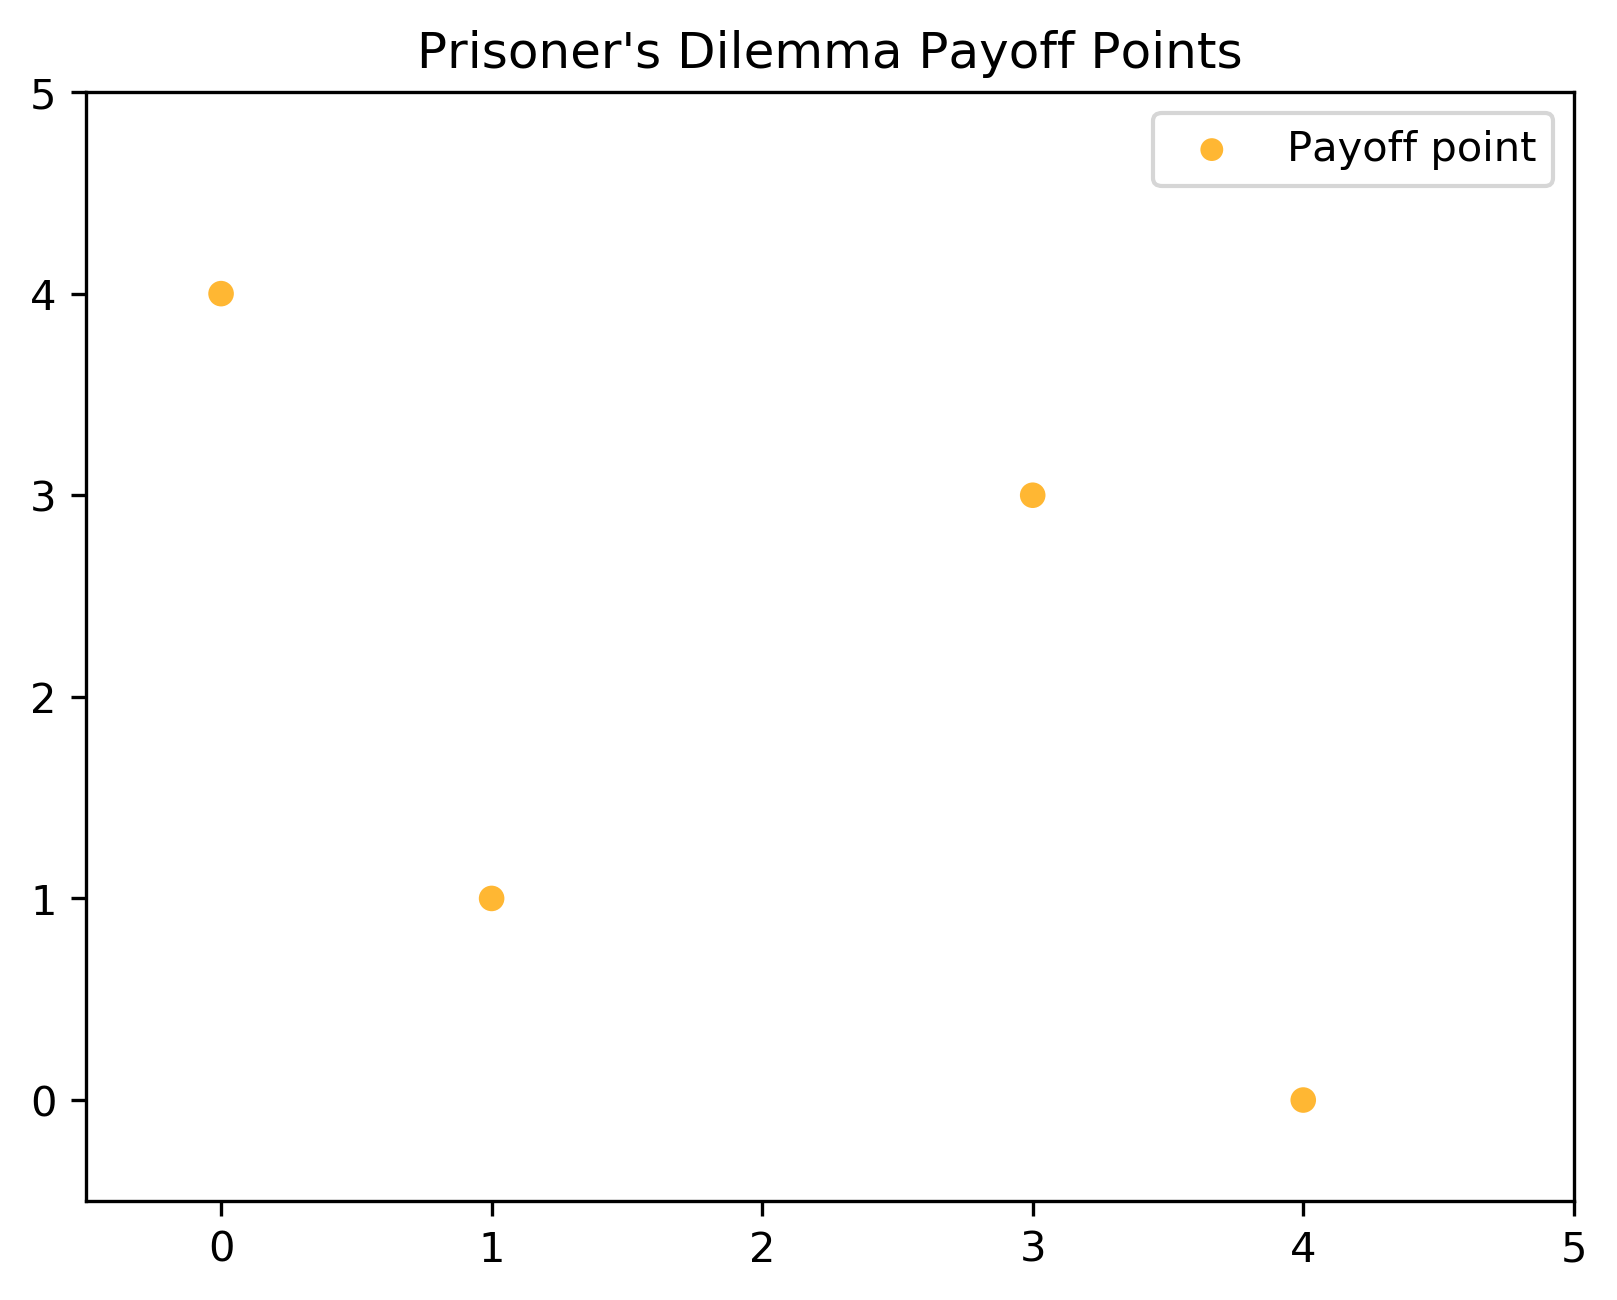
\includegraphics[scale=0.75]{resources/prisoners_dilemma_payoffs.png}
	\caption{The payoff points in a prisoner's dilemma game.}
	\label{prisoners_payoff_plot}
\end{figure}

\np The fact that limited invasions occur in this scenario makes sense when several facts about the model are considered:
\begin{enumerate}[label=(\alph*)]
	\item mutations can occur anywhere within the space and are small.
	\item the fitness of the agents (resident and mutant) is equal in areas of the surface not affected by the mutation.
	\item for a mutant to invade, they must achieve a fitness \textit{greater} than that achieved by the resident - as opposed to greater than or equal to.	
\end{enumerate} 
\np
So, if a mutation occurs at the point (2, 2), given that this mutation has a relatively small radius, 
the expected payoff of the mutant will not differ from that of the resident because the mutation does not touch any of the payoff points.
Hence, the fitnesses are equal, and no invasion occurs. Running large scale simulations using this model results in `utility surfaces' like figure \todo{prisoner's dillema run}.

\todo{is this to speculative/waffley?}
Intuitively, these non-meaningful results fit with out analogy of the utility surface in some way representing the real-world preferences of some agent.\
In reality, agents face many more kinds of situations than just one instance of a prisoner's dilemma,
and so to generate a preference surface that is potentially recognisable as one of a real-world agent it will need to be resilient to many different situations.


\chapter{Results \& Discussion}

\chapter{Conclusion}

\newpage

\bibliography{thesis}
\bibliographystyle{apalike}

\end{document}